\section{A Generalisation of the Helicoid}

In this section I will review \cite{BLR} a paper entitled \emph{A Generalization of the Helicoid} written by D. E. Blair and J. R. Vanstone in 1978.

We will begin by stating the theorem and then explaining what it means before giving an expanded version of the proof with more explanation than is given in \cite{BLR}.

\begin{nonumbertheorem}
Let $M^n$ be a complete minimal hypersurface of $E^{n+1}$ and suppose that $M^n$ admits a codimension 1 foliation by Euclidean $(n-1)$ spaces. Then either $M^n$ is totally geodesic or $M^n =  M^2 \times E^{n-2}$ where $M^2$ is a Helicoid in $E^3$.
\cite{BLR}
\end{nonumbertheorem}

Clearly a good place to start is with some definitions!

\subsection{Definitions}

\begin{definition}[Complete]
A surface which has no edges.
\end{definition}

\begin{definition}[Hypersurface]
A hypersurface is a generalization of a 2 dimensional surface to an n-dimensional surface embedded in (n+1)-dimensional space.

They are the set of the solutions to the equation:

\begin{displaymath}
f(x_1 + x_2 + ... + x_n) = 0 \mbox{\ \ \ \ embedded in } E^{n+1}
\end{displaymath}

\end{definition}

\begin{definition}[Codimension]
The codimension is the difference between the dimension of one (geometric or algebraic) object and the dimension of a smaller object contained in it.
\end{definition}

\begin{definition}[Foliation]
The idea of a foliation is easiest to grasp in $E^2$ and $E^3$ dimension to begin with.
For instance if we take $E^2$ minus the origin then a series of concentric circles foliate this space.
Likewise in $E^3$ minus the origin taking a series on concentric spheres foliates this space.
So the theorem requires that there exists a foliation of $M^n$ by objects of dimension $(n-1)$
\end{definition}

\begin{definition}[Totally Geodesic]
A hypersurface is totally geodesic if all of its geodesics are also geodesics of the ambient space.
\end{definition}

The theorem is therefore saying that if we have a hypersurface $M^n$ that we can foliate with objects of dimension $(n-1)$ then either $M^n$ is totally geodesic or $M^n = M^2 \times R^{n-2}$ where $M^2$ is a Helicoid in $E^3$

The exciting thing about this theorem is that it is in fact an extension of theorem \ref{Ruled} which says that in $E^3$ the only ruled surface apart from the plane is a Helicoid. A ruled surface (dimension n=2) is one that can be foliated by straight lines (dimension n=1) therefore a ruled surface admits a codimension 1 foliation. According to our theorem then such a minimal surface must either be totally geodesic which in $mathbb R^3$ means it has to be the plane or $M^2 \times E^0 = M^2$ which is the Helicoid.


\subsection{Necessary Tools for the Proof}
Before we begin to get to grips with the proof we need to review and introduce some notation and some tools.

\begin{enumerate}
	\item The Lie bracket $[X,Y] = \mathbf D_X Y - \mathbf D_Y X$
	\item If $(x^1,...,x^n)$ is a coordinate system then $\left[ \frac{\partial}{\partial x^i},\frac{\partial}{\partial x^j} \right] = 0$ - commuting partial derivatives.
	\item If $X,Y$ are uniform and tangential to a foliation then $[X,Y]$ is also tangential to the foliation
\end{enumerate}

We also need some rules for manipulating covariant derivatives.

$\mathbf D_x Y$ is linear in $X$ so
\begin{itemize}
	\item $\mathbf D_{X+Z}Y = \mathbf D_x Y + \mathbf D_z Y$
	\item $\mathbf D_{\alpha X}Y = \alpha \mathbf D_x Y$
	\item $\mathbf D_x(Y_1+Y_2)=\mathbf D_x Y_1 + \mathbf D_x Y_2$
	\item $\mathbf D_{\frac{\partial}{\partial X^i}} (\alpha Y) = \frac{\partial \alpha}{\partial X^i} Y + \alpha \mathbf D_{\frac{\partial}{\partial X^i}} Y$
\end{itemize}

\subsection{The Proof}
Firstly we need to set up some notation.

Let D be the Riemannian connection on $E^{n+1}$ and by $g$ and $\nabla$ the induced Riemannian metric and connection on $M^n$.

We'll use local coordinates $(t,x^1,...,x^n)$ such that

\begin{displaymath}
X_i = \frac{\partial}{\partial x^i} \mbox{\, \, \, \,} U = \alpha \frac{\partial}{\partial t}
\end{displaymath}
for some function $\alpha$
where $U$ is a unit vector field which together with $X_i$ forms and orthonormal basis such that $\mathbf D_{X_i}X_j = 0$

At this point we need to note an important difference between the notation we will use and the notation that the papers authors use. In their original paper they have coordinates $(t,x^2,...,x^n)$ and then every time they sum over the $x_i$'s they use $\sum_{i=2}^n$. Instead we will use standard \emph{Einstein Summation Notation} e.g. summing over repeated indices. Therefore indices will run from 1 to n unless otherwise specified (note that for convenience, in places $X_0 = \frac{\partial \ }{\partial t}$).

Then calculating the Lie bracket for this distribution 
\begin{eqnarray}
\nonumber
[U, Xi] &=& \mathbf D_U X_i - \mathbf D_{X_i} U \\
\nonumber
&=& \mathbf D_{\alpha \frac{\partial}{\partial t}} \frac{\partial}{\partial x^i} - \mathbf D_{\frac{\partial}{\partial x^i}}  \alpha \frac{\partial}{\partial t} \\
\nonumber
&=& \alpha \mathbf D_{\frac{\partial}{\partial t}}\frac{\partial}{\partial x^i}- \frac{\partial \alpha}{\partial x^i}\frac{\partial}{\partial t} - \alpha \mathbf D_{\frac{\partial}{\partial x^i}}\frac{\partial}{\partial t} \\
\nonumber
&=& \alpha \left[\frac{\partial}{\partial t},\frac{\partial}{\partial x^i}\right] - \frac{\partial \alpha}{\partial x^i}\frac{\partial}{\partial t} \\
\nonumber
&=& - \frac{\partial \alpha}{\partial x^i}\frac{\partial}{\partial t} \\
\nonumber
&=& - \frac{\partial \ln \alpha}{\partial x^i}\alpha\frac{\partial}{\partial t} \mbox{\ \ \ \ Letting } p = \ln \alpha \\
\nonumber
&=& -(X_i p)X
\end{eqnarray}

\begin{equation}
\framebox{$[U,X_i] = -(X_i p)U$ \ \ \ \ where $p = \ln \alpha$} 
\label{IntUXi}
\end{equation}

Since $(X_ip)U$ is tangential to the distribution, this means that the distribution is integrable. Basically this allows us to say that the distribution is \emph{smooth} and so the distribution is in fact a foliation.

Given the above coordinates and vector fields we can construct a metric:
\begin{eqnarray}
\nonumber
g_{00}&=&\frac{\partial}{\partial t} \cdot \frac{\partial}{\partial t} = \frac{1}{\alpha^2}|U|= \frac{1}{\alpha^2} \mbox{ since U is a unit vector field.} \\
\nonumber
\mbox{For $\mu \neq \nu$ } g_{\mu \nu}&=&\frac{\partial}{\partial x^\mu} \cdot \frac{\partial}{\partial x^\nu} = 0 \mbox{ since orthonormal.} \\
\nonumber
\mbox{For $\mu=\nu > 1$ } g_{\mu \nu}&=&\frac{\partial}{\partial x^\mu} \cdot \frac{\partial}{\partial x^\nu} = 1 \mbox{ since $X_j$ are unit vector fields.}
\end{eqnarray}
Giving
\begin{displaymath}
g_{\mu \nu} = 
\left(\begin{array}{clrrrr}      
\frac{1}{\alpha^2} &   &  &  &  & 0\\       
  								 & 1 &   & & &  \\ 
  								 &   & . &  & &  \\ 
  								 &   &   & . &  &  \\ 
  								 &   &   &   & . &  \\ 
  		0						 &  &  & & & 1  
\end{array}\right)
\mbox{\, \, \, \,} g^{\mu \nu} = 
\left(\begin{array}{clrrrr}      
\alpha^2 &   &  &  &  & 0\\       
  								 & 1 &   & & &  \\ 
  								 &   & . &  & &  \\ 
  								 &   &   & . &  &  \\ 
  								 &   &   &   & . &  \\ 
  		0						 &  &  & & & 1  
\end{array}\right)
\end{displaymath}

We now wish to calculate the $\nabla$ connections which are covariant derivatives on $M^n$.

To do this we use \emph{Theorem Egregium} to express everything in terms of the first fundamental form.

In particular we'll use the following:

\begin{equation}
\framebox{$\nabla_{X_i}X_j = \Gamma^k_{ij}X_k = \Gamma_{ijl}g^{lk}X_k = \frac{1}{2}(g_{il,j}+g_{jl,i}-g_{ij,l})g^{lk}X_k$}
\end{equation}

\begin{eqnarray}
\nonumber
\nabla_{X_i}X_j &=& \nabla_{\frac{\partial}{\partial x^i}}\frac{\partial}{\partial x^j} \\
\nonumber 
&=& \Gamma_{ij}^kX_k \\
\nonumber
&=& \Gamma_{ijl}g^{lk}X_k \\
\nonumber
&=& \frac{1}{2}(g_{il,j}+g_{jl,i}-g_{ij,l})g^{lk}X_k \mbox{\, \, \, $g^{\mu\nu}=0$ for $\mu \neq \nu$}\\
\nonumber
&=& \frac{1}{2}(g_{ik,j}+g_{jk,i}-g_{ij,k})g^{kk}X_k \\
\nonumber
&=& \frac{1}{2}(1_j+1_i-1_k)g^{kk}X_k \\
\nonumber
&=& 0
\end{eqnarray}
\begin{equation}
\framebox{$\nabla_{X_i}X_j = 0$}
\label{nXX}
\end{equation}

\begin{eqnarray}
\nonumber
\nabla_{X_i}U &=& \frac{\partial \alpha }{\partial x^i}  \frac{\partial}{\partial t} + \alpha \nabla_{\frac{\partial}{\partial x^i}}{\frac{\partial}{\partial t}} \\
\nonumber
&=& \frac{\partial \alpha }{\partial x^i}  \frac{\partial}{\partial t} + \alpha \Gamma^k_{i0}X_k \\
\nonumber
&=& \frac{\partial \alpha }{\partial x^i}  \frac{\partial}{\partial t} + \alpha \Gamma^{i0l}g^{lk}X_k \\
\nonumber
&=& \frac{\partial \alpha }{\partial x^i}  \frac{\partial}{\partial t} + \frac{\alpha}{2}(g_{il,0}+g_{0l,i}-g_{i0,l})g^{lk}X_k \\
\nonumber
&=& \frac{\partial \alpha }{\partial x^i}  \frac{\partial}{\partial t} + \frac{\alpha}{2}(g_{00,i}g^{00})X_0 \\
\nonumber
&=& \frac{\partial \alpha }{\partial x^i} \frac{\partial}{\partial t} + \frac{1}{2}\frac{\partial \frac{1}{\alpha^2}} {\partial x^i}\alpha^3\frac{\partial}{\partial t} \\
\nonumber
&=& \frac{\partial \alpha }{\partial x^i} \frac{\partial}{\partial t} - \frac{\partial \alpha} {\partial x^i}\frac{\partial}{\partial t} \\
\nonumber
&=& 0
\end{eqnarray}
\begin{equation}
\framebox{$\nabla_{X_i}U = 0$}
\label{nXU}
\end{equation}

\begin{eqnarray}
\nonumber
\nabla_UX_i &=& \nabla_{\alpha \frac{\partial}{\partial t}} \frac{\partial}{\partial x^i} \\ 
\nonumber
&=& \alpha \nabla_{\frac{\partial}{\partial t}}\frac{\partial}{\partial x^i} \\
\nonumber
&=& \alpha \Gamma_{0j}^k X_k \\
\nonumber
&=& \alpha \Gamma_{ijl}g^{lk} X_k \\
\nonumber
&=& \alpha \frac{1}{2}\left(g_{0l,j}+g_{jl,0}-g_{0j,l}\right)g^{lk} X_k \\
\nonumber
&=& \alpha \frac{1}{2}g_{00,j}g^{0k} X_k \mbox{\ \ \ \ (All $g_{ik,j}=0$ except for $g_{00,k}$) }\\
\nonumber
&=& \frac{\alpha}{2}\left[\frac{\partial}{\partial x^j}(\frac{1}{\alpha^2}) \alpha^2 \frac{\partial}{\partial t} \right] \\
\nonumber
&=& \frac{\alpha^2}{2}\left[\frac{\partial}{\partial x^j}(\frac{1}{\alpha^2}) X \right] \\
\nonumber
&=& \frac{1}{\alpha}\left[\frac{\partial \alpha}{\partial x^j} X \right] \\
\nonumber
&=& -\frac{1}{\alpha}\left[\frac{\partial \ln \alpha}{\partial x^j} \alpha X \right] \\
\nonumber
&=& - p_i X
\end{eqnarray}

\begin{equation}
\framebox{$\nabla_{U}X_i = -p_i X$}
\label{nUX}
\end{equation}

\begin{eqnarray}
\nonumber
\nabla_{U} U &=& \nabla_{\alpha \frac{\partial \ }{\partial t}}{\frac{\partial}\partial t} \\
\nonumber
&=&\alpha\nabla_{\frac{\partial \ }{\partial t}}\alpha \frac{\partial \ }{\partial t} \\
&=& \alpha \left[ \frac{\partial \alpha}{\partial t} \frac{\partial \ }{\partial t} + \alpha \mbox{\framebox{$\nabla_{\frac{\partial \ }{\partial t}}{\frac{\partial \ }{\partial t}}$}} \right ] \label{ntt}
\end{eqnarray}

Expanding the boxed covariant derivative:

\begin{eqnarray}
\nonumber
\nabla_{\frac{\partial \ }{\partial t}}{\frac{\partial \ }{\partial t}} &=& \Gamma_{00}^k X_k \\
\nonumber
&=& \Gamma_{00l}g^{lk}X_k \\
\nonumber
&=& \frac{1}{2}(g_{00,l}+g_{0l,0}-g{00,l})g^{lk}X_k \\
\nonumber
&=& \frac{1}{2} \left[g_{00,0}g^{00}X_0 - g_{00,1}g^{11} X_1 \ldots - g_{00,n}g^{nn} X_n \right] \\
\nonumber
&=& \frac{1}{2}\frac{\partial \ }{\partial t}\left(\frac{1}{\alpha^2}\right)\alpha^2\frac{\partial \ }{\partial t} - \frac{1}{2}  \frac{\partial \ }{\partial x^i}\left(\frac{1}{\alpha^2}\right)X_i \\
\nonumber
&=& -\frac{1}{\alpha}\frac{\partial \alpha}{\partial t}\frac{\partial \ }{\partial t} + \frac{1}{\alpha^3}\frac{\partial \alpha}{\partial x^i} X_i \\
\nonumber
&=& -\frac{1}{\alpha}\frac{\partial \alpha}{\partial t}\frac{\partial \ }{\partial t} + \frac{1}{\alpha^2}\frac{\partial \ln \alpha}{\partial x^i} X_i \\
\nonumber
&=& -\frac{1}{\alpha}\frac{\partial \alpha}{\partial t}\frac{\partial \ }{\partial t} + \frac{1}{\alpha^2} p_i X_i \\
\end{eqnarray}

Subbing this back in to \ref{ntt} gives us:

\begin{eqnarray}
\nonumber
\nabla_{U} U &=& \alpha \left[ \frac{\partial \alpha}{\partial t} \frac{\partial \ }{\partial t} + \alpha \mbox{\framebox{$\nabla_{\frac{\partial \ }{\partial t}}{\frac{\partial \ }{\partial t}}$}} \right ]  \\
\nonumber
&=& p_i X_i
\end{eqnarray}

\begin{equation}
\framebox{$\nabla_{U}U = p_i X_i$}
\label{nUU}
\end{equation}

We now introduce the Weingarten map which we define as

\begin{definition}[The Weingarten Map]
\begin{displaymath}
A(Y) = D_{\mathbf Y}\mathbf N
\end{displaymath}
\end{definition}

Now we apply the Weingarten map to our coordinates and expand via a basis expansion giving

\begin{equation}
\framebox{$A(U) = rU + q_i X_i, \ \ \ \ A (X_i) = q_i U$}
\label{Weingarten}
\end{equation}

Where $r$ and $q_i$ are some constants. We will use inner products to show that the $q_i$'s in both equations are equal and that $A(X_i)$ has zero $X_i$ component as shown. We can do this since $M^n$ is foliated by Euclidean (n-1)-dimensional spaces.

\begin{eqnarray}
\nonumber
<A(X_i), X_j> &=& <D_{X_i} \mathbf N, X_j> \\
\nonumber
&=& -<\mathbf N, D_{X_i}X_j> = 0
\end{eqnarray}

To show the $q_i$'s are the same in both equations we show
\begin{displaymath}
<A(X_i), U> = <A(U),X_i>
\end{displaymath}

So

\begin{eqnarray}
\nonumber
<A(X_i), U> &=& <D_{X_i} \mathbf N, U> \\
\nonumber
&=& -<N, D_{X_i}U> \\
\nonumber 
&=& -<N, D_U X_i - [U,X_i]>\\
\nonumber
&=& -<N, D_U X_i + X_i p U>\\
\nonumber
&=& -<N, D_U X_i>\\
\nonumber
&=& -<D_U N, X_i>
\end{eqnarray}

\begin{definition}[The Codazzi Equation]
\begin{displaymath}
(\nabla_X A)Y - (\nabla_{Y} A)X = 0
\end{displaymath}
For vector fields X and Y.

Where 
\begin{itemize}
	\item $(\nabla_X A) Y = \nabla_X(AY) - A(\nabla_X Y)$
	\item $(\nabla_Y A) X = \nabla_Y(AX) - A(\nabla_Y X)$
\end{itemize}
\end{definition}

So in our basis $(\nabla_U A) X_i - (\nabla_{X_i} A) U = 0$.

Plugging in from the definition and results shown previously:

\begin{align}
\nonumber
&\Leftrightarrow& &\nabla_U(AX_i)-A(\nabla_UX_i)-\nabla_{X_i}(AU)+A(\nabla_{X_i}U)& &=& &0& \\
\nonumber
&\Leftrightarrow& &\nabla_U(q_i U) - A(-p_i U) - \nabla_{X_i}(rU+ q_jX_j) + A(0)& &=& &0& \\
\nonumber
&\Leftrightarrow& &U(q_i)U+q_i\nabla_UU+p_iA(U) -\nabla_{X_i}rU-\nabla_{X_i}q_jX_j& &=& &0&\\
\nonumber
&\Leftrightarrow& &U(q_i)U+q_i\nabla_UU+p_iA(U) - X_irU  & &\ & &\ & \\
\nonumber
&\ & & \ \ \ \ \ \ \ \ \ \ \ \ \ \ \ \ \ \ - r\nabla_{X_i}U-X_iq_jX_j-q_j\nabla_{X_i}X_j& &=& &0& \\
\nonumber
&\Leftrightarrow& &Uq_iU - X_irU+q_ip_jX_j + p_i(rU+q_jX_j)-X_iq_jX_j& &=& &0& \\
\nonumber
&\Leftrightarrow& &[Uq_i + rp_i-X_ir]U+[q_ip_j+p_iq_j-X_iq_j]X_j& &=& &0&
\end{align}

Since $X_i$ and $U$ form a basis, they are linearly independent and so
\begin{equation}
\framebox{$X_ir - Uq_i - rp_i = 0 \ \ \ \ X_iq_j-q_ip_j-p_iq_j=0$}
\label{Codazzi}
\end{equation}

Clearly then 
\begin{equation}
\framebox{$X_iq_j - X_jq_i = 0$}
\label{Xiqjcom}
\end{equation}

\begin{definition}[The Gauss Equation]
\begin{displaymath}
R(X,Y)Z=g(AY,Z)AX-g(AX,Z)AY
\end{displaymath}
For vector fields X,Y and Z. Where R is the Riemann curvature tensor and A is the Weingarten map.
\end{definition}

\begin{aside}[The Gauss Equation in $E^3$, \cite{HIC}]

While not required for the proof it is interesting to realise that the Gauss equation a generalised version of the Gauss Curvature in $E^3$.

Let $\mathbf x_u$ and $\mathbf x_v$ be an orthonormal base for a surface in $E^3$. Then we claim that $K(p) = \mbox{ Det }A_p = g(R(\mathbf x_u,\mathbf x_v)\mathbf x_v,\mathbf x_u)$.

Remembering that since $\mathbf x_u$ and $\mathbf x_v$ are orthonormal $EG-F^2 = 1$ the proof follows as:

\begin{eqnarray}
\nonumber
\mbox{Det }A_p &=& g(R(\mathbf x_u,\mathbf x_v)\mathbf x_v,\mathbf x_u) \\
\nonumber
&=& g(g(A\mathbf x_v,\mathbf x_v)A\mathbf x_u - g(A\mathbf x_u,\mathbf x_v)A\mathbf x_v,\mathbf x_u) \\
\nonumber
&=& g(A\mathbf x_v,\mathbf x_v)g(A\mathbf x_u,\mathbf x_u) - g(A\mathbf x_u,\mathbf x_v)g(A\mathbf x_v,\mathbf x_u) \\
\nonumber
&=&g(\mathbf N,D_{\mathbf x_v}\mathbf x_v)g(\mathbf N,D_{\mathbf x_u}\mathbf x_u) - g(\mathbf N, D_{\mathbf x_u}\mathbf x_v)g(\mathbf N, D_{\mathbf x_v}\mathbf x_u) \\
\nonumber
&=&g(\mathbf N,X_{vv})g(\mathbf N,X_{uu}) - g(\mathbf N, X_{uv})g(\mathbf N, X_{uv})\\
\nonumber
&=& LN - M^2 = K \mbox{\ \ \ \ From equation \ref{equ:K}}
\end{eqnarray}
\end{aside}


From this we can generate a final equation which together with the equations we produced from the Codazzi equation completely determine the dependence of the $p_i$ and $q_i$ on the $x^i$ in a tubular neighbourhood, T, of any leaf.

We start from $R(X_i,U)U = g(AU,U)AX_i-g(AX_i,U)AU$ and take the inner product of both sides with respect to $X_j$.

So
\begin{eqnarray}
\nonumber
RHS &=& g(R(X_i,U)U,X_j)\\
\nonumber
&=& g(\nabla_{X_i}\nabla_{U}U - \nabla_U\nabla_{X_i}X_j-\nabla_{[X_i,U]}U, X_j) \\
\nonumber
&=&g(\nabla_{X_i}(p_kX_k)-\nabla_U(0)-\nabla_{(X_ip)U}U, X_j) \\
\nonumber
&=&g((X_ip_k)X_k + p_k\nabla_{X_i}X_k -(X_ip)\nabla_UU - U\nabla_{X_ip}U,X_j) \\
\nonumber
&=&g((X_ip_k)X_k + p_k\nabla_{X_i}X_k-(X_ip)p_iX_i - U\nabla_{X_ip}U,X_j) \\
\nonumber
&=&g((X_ip_k)X_k -(X_ip)p_iX_i,X_j) \\
\nonumber
&=&X_ip_k-(X_ip)p_j \\
\nonumber
&=&X_ip_k-p_ip_j
\end{eqnarray}

\begin{eqnarray}
\nonumber
LHS &=& g(g(AU,U)AX_i - g(AX_i,U)AU),X_j) \\
\nonumber
&=& g(AU,U)g(AX_i,X_j)-g(AX_i,U)g(AU,X_j) \\
\nonumber
&=& g(rU,q_iX_i, U)g(0,X_j)-g(q_iU,U)g(rU+q_iX_i, X_j) \\
\nonumber
&=& -g(q_iU,U)g(q_jX_j,X_i) \\
\nonumber
&=& -q_iq_j 
\end{eqnarray}

$\therefore$

\begin{equation}
\framebox{$X_ip_j = p_ip_j - q_iq_j$}
\label{GaussEq}
\end{equation}

If $\omega$ is the 1-form defined by $\omega(U) = r$ for some function $\omega(X_i)=q_i$ on T. Then
\begin{eqnarray}
\nonumber
d\omega(U,X_i)&=&\frac{1}{2}(Uq_i-X_ir+rp_i)=0 \\
\nonumber
d\omega(X_i, X_j)&=&\frac{1}{2}(X_iq_j-X_jq_i)=0 \\
\end{eqnarray}

This means $\omega$ is closed. Therefore since the leaves of the foliation are simply-connected, $\omega = dq$ for some function q on T.

We now again use complex analysis to continue with the proof. First we define a complex-valued function $s$ on $T$ by $s=p+iq$, then we can use the Gauss-Codazzi equations to show the following:

\begin{eqnarray}
\nonumber
X_iX_j(s) &=& X_i(X_jp + iX_jq) \\
\nonumber
&=& X_i(p_j+iq_j)\\
\nonumber
&=& X_ip_j+iX_iq_j \\
\nonumber
&=&p_ip_j-q_iq_j+i(p_iq_j+q_ip_j) \\
\nonumber
&=&(p_i+iq_i)(p_j+iq_j) \\
\nonumber
&=&X_i(p+iq)X_j(p+iq) \\
\nonumber
&=& (X_is)(X_js)
\end{eqnarray}

\begin{equation}
\framebox{$X_iX_js=(X_is)(X_js)$}
\label{X_iX_js}
\end{equation}

Alternatively if we let $S=e^{-s}$
\begin{eqnarray}
\nonumber
X_iX_jS &=& X_iX_je^{-s}  \\
\nonumber
&=&X_i(X_j(-s)e^{-s}) \\
\nonumber
&=&X_i(X_j(-s))e^{-s}+X_j(-s)X_i(-s)e^{-s} \\
\nonumber
&=& X_iX_j(-p-iq)S+X_j(-p-iq)X_i(-p-iq)S \\
\nonumber
&=& X_i(-p_j-iq_j)S+(-p_j-iq_j)(-p_i-iq_i)S \\
\nonumber
&\ &\mbox{Subbing in from Gauss/Codazzi equations:} \\
\nonumber
&=&(-(p_ip_j-q_iq_j)-i(p_iq_j+q_ip_j))S+(-p_j-iq_j)(-p_i-iq_i)S \\
\nonumber
&=&S(\cancel{-p_ip_j}+\cancel{q_iq_j}-\cancel{i p_iq_j}-\cancel{i q_ip_j}+\cancel{p_jp_i}+\cancel{ip_jq_i}+\cancel{iq_jp_i}-\cancel{q_jq_i}) = 0
\end{eqnarray}
\begin{equation}
\framebox{$X_iX_jS=0$}
\label{X_iX_jS}
\end{equation}

The general solution of this system is
\begin{equation}
\framebox{$S = \tau_0 + \tau_ix^i $}
\label{genSol}
\end{equation}

where $\tau_0$, $\tau_i$ are complex valued functions of t. 

If we assume all the $\tau_i$ vanish S becomes a function of t only and therefore $X_is = 0$. Since $s=p+iq$ it follows that $X_is = p_i+iq_i = 0$ and so the $p_i$ and $q_i$ vanish as well.

Given this, the Weingarten map (\ref{Weingarten}) becomes 
\begin{equation}
\framebox{$AU = rU$, $AX_i = 0$}
\label{equ:A}
\end{equation}

We now apply the condition that $M^n$ be minimal. In section (\ref{MeanCurve}) the mean curvature was shown to be $\frac{1}{2}\mbox{Trace }d\mathbf N_p$. $d\mathbf N_p$ is in fact the Weingarten map. So if $M^n$ is minimal, $\mbox{Trace }A=0$ which means $r=0$, therefore A becomes zero at all points from equation \ref{equ:A} which implies that $M^n$ is totally geodesic and so we have proved the totally geodesic case of the theorem.

The other case occurs when some $\tau_i \neq 0$. In this case, neither $e^s$ or$S$ ever vanish. Therefore the $\tau_i$ are linearly dependent over $\mathbb R$ and so $S$ has the form

\begin{displaymath}
S=\tau_0+\tau l(x)
\end{displaymath}

where ${\tau_0, \tau}$ are linearly independent over $\mathbb R$ and depend only on t, while l is the real valued linear form

\begin{displaymath}
l(x) = l_ix^i
\end{displaymath}

We proceed by taking $e^{-(p+iq)} = \tau_0 + \tau l$ and acting $X_i$ on both sides.

\begin{eqnarray}
\nonumber
e^{-(p+iq)} &=& \tau_0 + \tau l \\
\nonumber
\Leftrightarrow -p-iq&=& \ln (\tau_0+\tau l) \\
\nonumber
\stackrel{X_i}{\Leftrightarrow} -p_i-iq_i &=& \frac{\tau l_i}{\tau_0+\tau l} \\
\nonumber
&=& \frac{\cancel{\tau}l_i}{\cancel{\tau}(\frac{\tau_0}{\tau}+l)}\\
\nonumber
&=& \frac{l_i}{\sigma + l} \mbox{\ \ \ \ Letting $\sigma = \frac{\tau_0}{\tau}$}
\end{eqnarray}

So now taking the real and imaginary parts:
\begin{eqnarray}
\nonumber
p_i &=& \Re\frac{-l_i}{\sigma+l} \\
\nonumber
&=& \Re\frac{l_i(\bar{\sigma}+l)}{(\sigma+l)(\bar{\sigma}+l)} \\
\nonumber
&=& \Re \frac{-l_i(\bar{\sigma} + l)}{|\sigma+l|^2} \\
\nonumber
&=& \frac{-l_i}{|\sigma+l|^2}(l+\Re \sigma)
\end{eqnarray}

\begin{eqnarray}
\nonumber
q_i &=& \Im \frac{-l_i}{\sigma + l} \\
\nonumber
&=& \Im \frac{-l_i(\bar{\sigma} +l)}{(\sigma} +l)(\bar{\sigma} +l) \\
\nonumber
&=& \Im \frac{-l_i\bar{\sigma} - l_il}{|\sigma+l|^2} \\
\nonumber
&=&\frac{-l_i\Im\bar{\sigma}}{|\sigma+l|^2} \\
\nonumber
&=&\frac{l_i\Im\sigma}{|\sigma+l|^2}
\end{eqnarray}

\begin{equation}
\framebox{$p_i = \frac{-l_i}{|\sigma+l|^2}(l+\Re \sigma) \ \ \ \ q_i = \frac{l_i\Im\sigma}{|\sigma+l|^2}$}
\label{piqi}
\end{equation}

From these we can write $p_i$ in terms of $q_i$
\begin{displaymath}
p_i = \frac{-l_i}{|\sigma+l|^2}(l+\Re \sigma) = \frac{-l_i}{|\sigma+l|^2}(l+\Re \sigma) \frac{\Im \sigma}{\Im \sigma} = -\frac{(l+\Re \sigma)}{\Im \sigma}q_i
\end{displaymath} 

\begin{equation}
\framebox{$p_i =-\frac{(l+\Re \sigma)}{\Im \sigma}q_i$}
\label{pi=qi}
\end{equation}

We can now use \ref{pi=qi} to give 
\begin{equation}
\framebox{$\nabla_UU = p_iX_i = -\frac{(l+\Re \sigma)}{\Im \sigma}q_iX_i$}
\label{NUUq}
\end{equation}


and using the Codazzi  equation (\ref{Codazzi})for $X_iq_j$

\begin{eqnarray}
\nonumber
\nabla_{q_iX_i}(q_jX_j) &=& q_i \nabla_{X_i}q_jX_j \\
\nonumber
&=& q_i(X_i(q_j)X_j+q_j\cancelto{0}{\nabla_{X_i}X_j} \\
\nonumber
&=&q_iX_iq_jX_j \\
\nonumber
&=&q_i(p_iq_j+q_ip_j)X_j \\
\nonumber
&=&q_i(-\frac{l+\Re \sigma}{\Im \sigma}q_iq_j-q_i\frac{l+\Re \sigma}{\Im \sigma}q_j)X_j \\
\nonumber
&=& q_i(-2\frac{l+\Re \sigma}{\Im\sigma}q_iq_j)X_j \\
\nonumber
&=& -2\frac{l+\Re \sigma}{\Im\sigma}q_i^2q_jX_j
\end{eqnarray}

\begin{equation}
\framebox{$\nabla_{q_iX_i}(q_jX_j) = -2\frac{l+\Re \sigma}{\Im\sigma}q_i^2q_jX_j$}
\label{NqiXiqjXj}
\end{equation}

Completing to calculate the connections:

\begin{eqnarray}
\nonumber
\nabla_U q_iX_i &=& Uq_iX_i + q_i\nabla_UX_i \\
\nonumber
&=& Uq_iX_i + q_i\left(\frac{l+\Re \sigma}{\Im \sigma} \right)q_iU \\
&=& Uq_iX_i+ q_i^2 \frac{l+\Re \sigma}{\Im \sigma}
\label{NUqiXi}
\end{eqnarray}

and 

\begin{equation}
\nabla_{q_iX_i}U = q_i\nabla_{X_i}U = 0
\label{NqiXiU}
\end{equation}

Now again if $M^n$ is minimal, $r=0$ and hence from the Codazzi equation (\ref{Codazzi}) $Uq_i=0$ 

We have shown that $\nabla_UU$, $\nabla_Uq_iXi$, $\nabla_{q_iX_i}U$ and $\nabla_{ q_iX_i}q_iX_i$ are all linear combinations of the $U$ and $q_iX_i$ so we have a 2-dimensional distribution spanned by $U$ and $q_iX_i$. We will now show that is also integrable (e.g. the Lie bracket is tangential to the distribution).

\begin{eqnarray}
\nonumber
[U,q_iX_i] &=& D_Uq_iX_i - D_{q_iX_i}U \\
\nonumber
&=& (\cancelto{0}{Uq_i})\ X_i+q_i\left(D_UX_i-D_{X_i}U\right) \mbox{\ \ \ \ Since Minimal} \\
\nonumber
&=& q_i[U,X_i] \\
\nonumber
&=& -q_iX_ipU \mbox{\ \ \ \ (\ref{IntUXi})} \\
\nonumber
&=& -q_ip_iU
\end{eqnarray}

\begin{equation}
\framebox{$[U,q_iX_i]=-q_ip_iU$}
\label{IntUqiXi}
\end{equation}

Since this distribution is integrable and the connections are all linear combinations of $U$ and $q_iX_i$ it follows that the leaves $M^2$ of this foliation are totally geodesic in $M^n$

We define a complementary distribution such that Y and Z are vector fields tangential to our original distribution.

We now have $M^2 \subset M^n \subset E^{n+1}$ each of which have their own Riemannian connection as stated earlier. So $\mathbf D$ is the connection on $E^{n+1}$ and $\nabla$ is the connection on $M^n$. We will show how these connections are related to each other in the complementary distribution.

We proceed using a relation from Riemannian geometry:

\begin{equation}
\mathbf D_YZ-\nabla_YZ=<AY,Z>N
\end{equation}

\begin{eqnarray}
\nonumber
<AY,Z> &=& <\mathbf D_Y\mathbf N, Z> \\ 
\nonumber
&=& -<\mathbf N, \mathbf D_YZ> = 0 
\end{eqnarray}

This is because Y and Z are tangential to $M^2$ and so $\nabla_YZ$ is also tangential to $M^2$ and therefore normal to $\mathbf N$.

So 
\begin{equation}
\framebox{$\mathbf D_YZ=\nabla_YZ$}
\label{Connections}
\end{equation}

We also need $g(\nabla_YZ,U)$. Since $Y$ and $Z$ belong to the complementary distribution they are tangential to the original foliation by Euclidean spaces whose leaves are totally geodesic.  Therefore $\nabla_YZ$ is at least tangent to the leaves of the original foliation.  $U$ is the normal to the original foliation and therefore $g(\nabla_YZ,U)=0$
\begin{equation}
\framebox{$g(\nabla_YZ,U)=0$}
\label{gNyzU}
\end{equation}

Since $Y$ and $X_i$ are both tangential to the foliation, $Y$ can be written as a linear combination of the $X_i$ such that:

\begin{equation}
Y=b_jX_j
\end{equation}

Similarly we want to calculate $g(\nabla_YZ, q_iX_i)$

\begin{eqnarray}
\nonumber
g(\nabla_YZ,q_iX_i) &=& -g(Z,\nabla_Yq_iX_i) \\
\nonumber
&=& -g(Z,\nabla_{b_jX_j}q_iX_i) \\
\nonumber
&=& -g(Z,b_j(X_jq_i)X_i + b_jq_i\cancelto{0}{\nabla_{X_j}{X_i}}) \\
\nonumber
&=& -g(Z,b_jX_jq_iX_i) \\
\nonumber
&=& -g(Z,b_j(p_iq_j+q_ip_j)X_i) \\
\nonumber
&=& -g(Z,b_j\left(-\frac{l+\Re\sigma}{\Im \sigma}q_iq_j - q_j\frac{l+\Re\sigma}{\Im\sigma}q_i\right)X_i) \\
\nonumber
&=& -g(Z,b_j\left(-2\frac{l+\Re \sigma}{\Im \sigma}q_iq_j\right)X_i) \\
\nonumber
&=& 2\frac{l+\Re\sigma}{\Im \sigma}(b_jq_j)g(Z,q_iX_i) = 0 
\end{eqnarray}

So the complementary distribution is also integrable with integral sub-manifolds which are totally geodesic in both $M^n$ and $E^{n+1}$. It now follows that since $M^n$ is complete, $M^2$ lies in $E^3$. Then since $M^2$ is totally geodesic in $M^n$ it is minimal in $E^3$. Since $M^n = M^2 \times E^{n-2}$ is foliated by $(n-1)$-dimensional Euclidean spaces, $M^2$ must be a ruled surface and hence a Helicoid (Our classical result for ruled minimal surfaces, Theorem \ref{Ruled}).

\section{Visualising a Generalised Helicoid}
To round things off we will now attempt to visualise what $M^3$ looks like (that is a 3-Helicoid embedded in $E^4$).

Clearly we can't draw such an object but we can take slices through it. Suppose you were a 2-dimensional being, you could of course still mathematically create a 2-sphere which you could then illustrate to your contemporaries by taking slices through it and drawing a series of circles. They would start from a point, grow to fixed radius and then decrease back to a point. We shall use exactly the same method here except that our \emph{slices} are 3-dimensional objects.

So mathematically our 3-Helicoid is parametrised by:
\begin{displaymath}
\mathbf X(u,v,w) = (\sinh \: v\: cos \: u, \sinh \:v \: \sin \:u, u, w)
\end{displaymath}

If we fix w, and let u and v vary only looking at the first three coordinate functions we get our normal Helicoid - eg at every point w exists $M^2$.

If we fix u (arbitrarily at $\frac{\pi}{3}$)and ignore the obvious third coordinate, leaving:
\begin{displaymath}
\mathbf X(v,w) = (\sinh v \cos \frac{\pi}{3}, \sinh v \sin \frac{\pi}{3}, w)
\end{displaymath}

This gives a plane which rotates if we vary our choice of u. This can be seen in Figure \ref{fig:3HelFixedu}.
\begin{figure}[htbp]
	\centering
       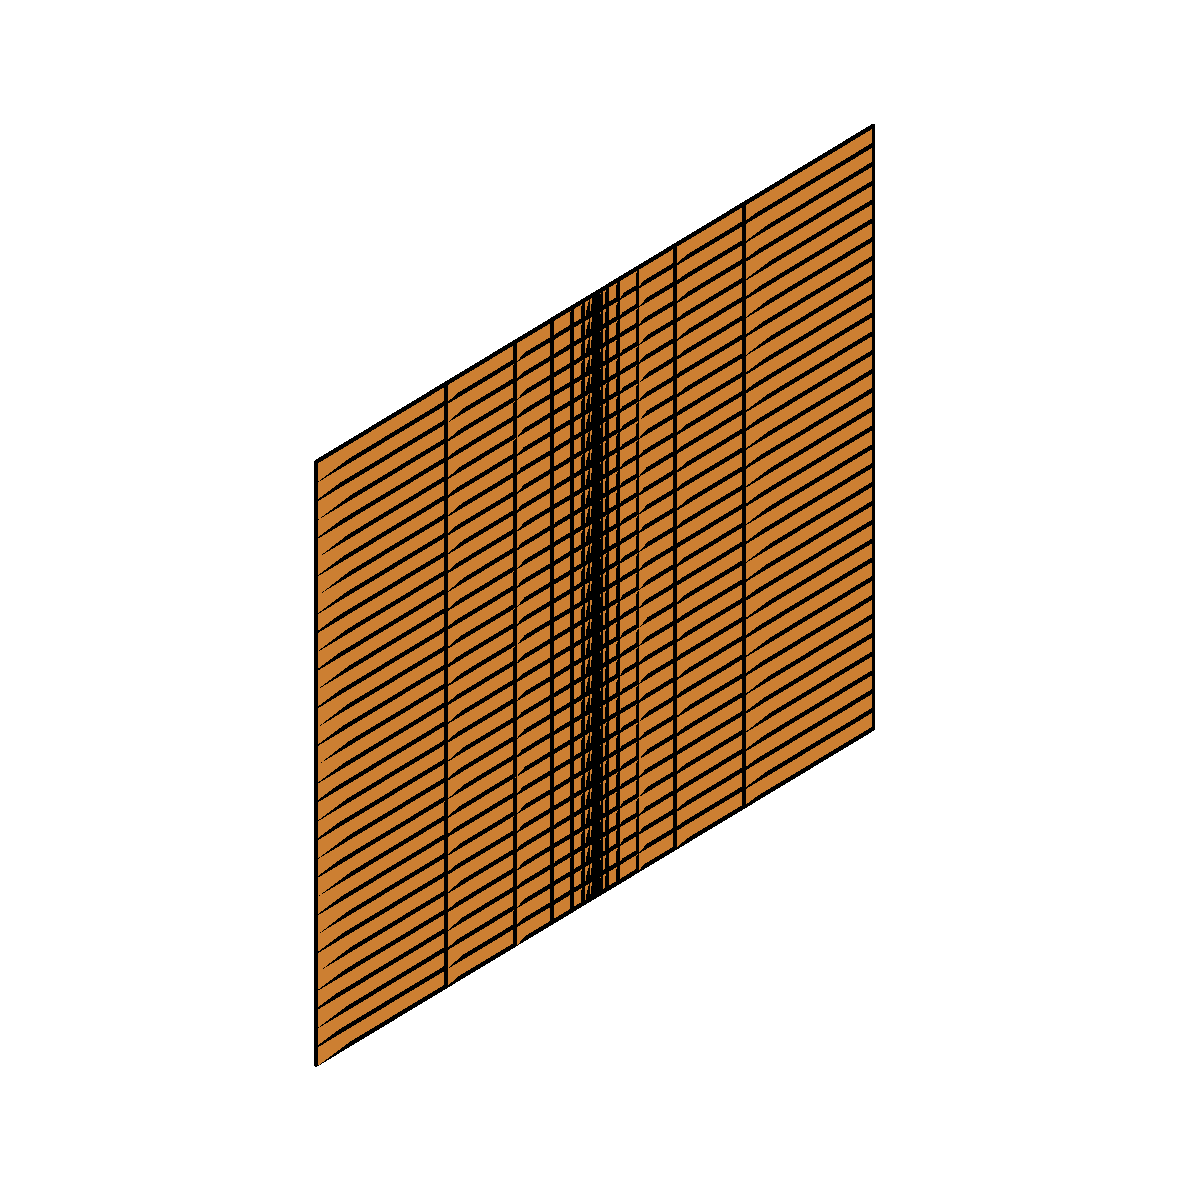
\includegraphics[width=8cm]{Images/3HelFixedu.eps}
   \caption{3-Helicoid with Fixed u}
   \label{fig:3HelFixedu}
\end{figure}

Similarly if we fix v (arbitrarily at $1$) and again ignore the third coordinate function leaving

\begin{displaymath}
\mathbf X(u,w) = (\sinh \: 1\: cos \: u, \sinh \:1 \: \sin \:\ u, w)
\end{displaymath}

This gives a cylinder whose radius increases if we increase the fixed value of v. This can be be seen in Figure \ref{fig:3HelFixedv}.
\begin{figure}[htbp]
	\centering
       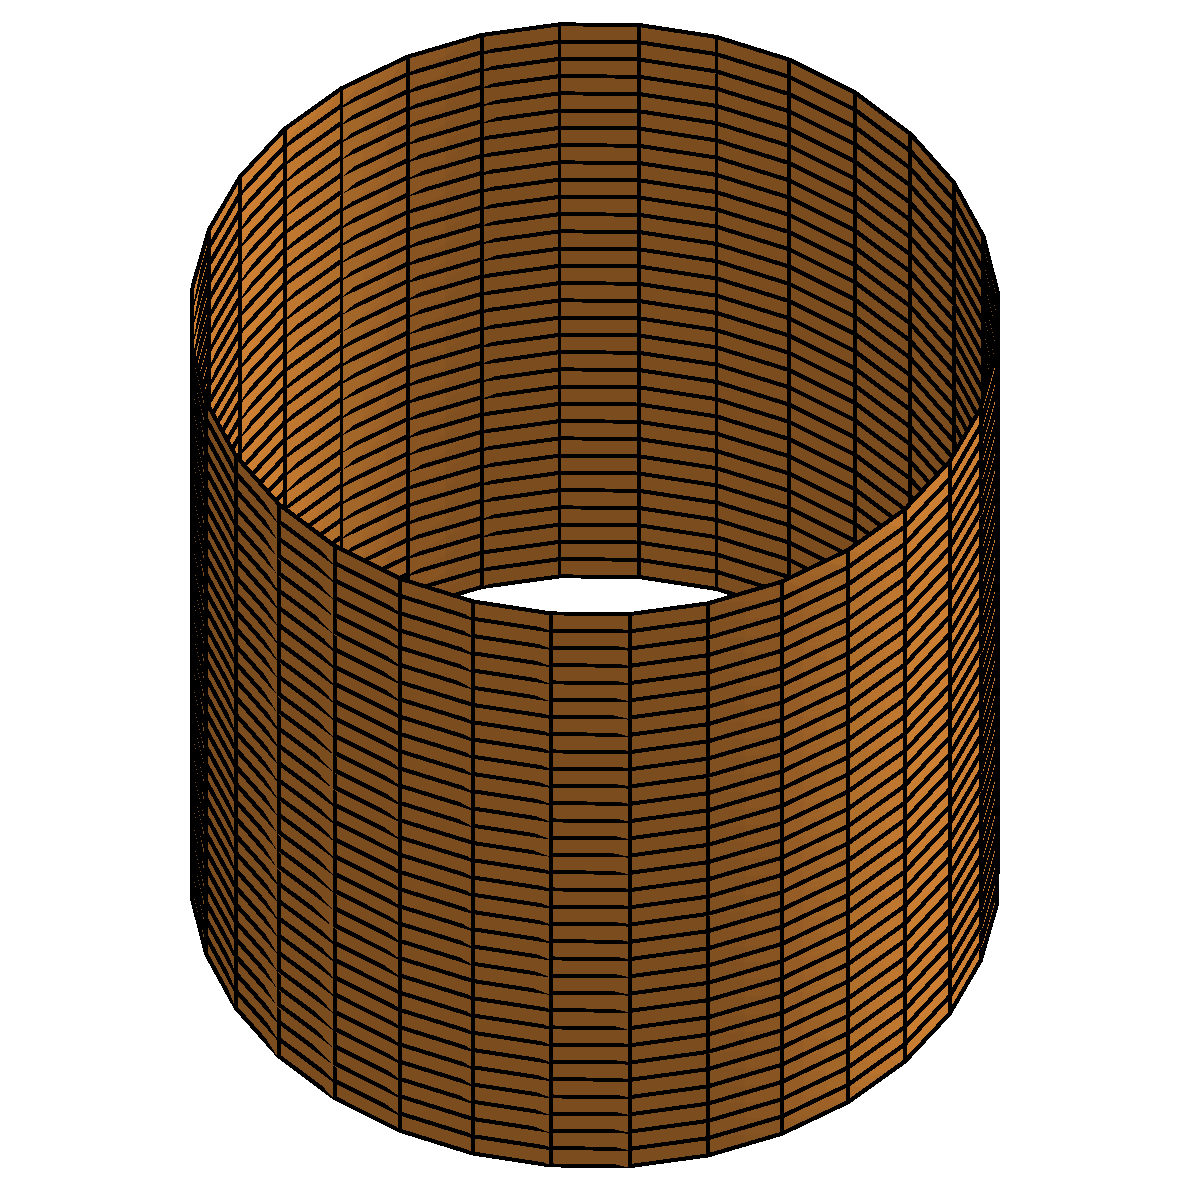
\includegraphics[width=8cm]{Images/3HelFixedv.eps}
   \caption{3-Helicoid with Fixed v}
   \label{fig:3HelFixedv}
\end{figure}

